
% Aberdeen style guide should be followed when using this
% layout. Their template powerpoint slide is used to extract the
% Aberdeen color and logo but is otherwise ignored (it has little or
% no formatting in it anyway).   
% 
% http://www.abdn.ac.uk/documents/style-guide.pdf

%%%%%%%%%%%%%%%%%%%% Document Class Settings %%%%%%%%%%%%%%%%%%%%%%%%%
% Pick if you want slides, or draft slides (no animations)
%%%%%%%%%%%%%%%%%%%%%%%%%%%%%%%%%%%%%%%%%%%%%%%%%%%%%%%%%%%%%%%%%%%%%%
%Normal document mode% 
\documentclass[10pt,compress,unknownkeysallowed]{beamer}
%Draft or handout mode 
%\documentclass[10pt,compress,handout,unknownkeysallowed]{beamer}
%\documentclass[10pt,compress,handout,ignorenonframetext,unknownkeysallowed]{beamer}


%%%%%%%%%%%%%%%%%%%% General Document settings %%%%%%%%%%%%%%%%%%%%%%%
% These settings must be set for each presentation
%%%%%%%%%%%%%%%%%%%%%%%%%%%%%%%%%%%%%%%%%%%%%%%%%%%%%%%%%%%%%%%%%%%%%%
\newcommand{\shortname}{jefferson.gomes@abdn.ac.uk}
\newcommand{\fullname}{Dr Jeff Gomes}
\institute{School of Engineering}
\newcommand{\emailaddress}{}%jefferson.gomes@abdn.ac.uk}
\newcommand{\logoimage}{../../FigBanner/UoAHorizBanner}
\title{Chemical Thermodynamics (EX3029)}
\subtitle{Module 4: Solution Thermodynamics}
\date[ ]{ }



%%%%%%%%%%%%%%%%%%%%%%%%%%%%%%%%%%%%%%%%%%%%%%%%%%%%%%%%%%%%%%%%%%%%%%%%%%%%%%%
% BABEL and LANGUAGES %%%%%%%%%%%%%%%%%%%%%%%%%%%%%%%%%%%%%%%%%%%%%%%%%%%%%%%%%
%%%%%%%%%%%%%%%%%%%%%%%%%%%%%%%%%%%%%%%%%%%%%%%%%%%%%%%%%%%%%%%%%%%%%%%%%%%%%%%
% \usepackage{listings}                   % it is a source code printer for LATEX
                                          % \lstset{language=Python}
                                          % \lstinputlisting{source.py}   % command used to pretty-print stand alone files
\usepackage[english]{babel}               % [french, frenchb, english, ]
    % http://forum.mathematex.net/latex-f6/les-puces-avec-babel-t4256.html
    % http://www.grappa.univ-lille3.fr/FAQ-LaTeX/11.1.html


%%%%%%%%%%%%%%%%%%%%%%%%%%%%%%%%%%%%%%%%%%%%%%%%%%%%%%%%%%%%%%%%%%%%%%%%%%%%%%%
% FONTS and ENCODING %%%%%%%%%%%%%%%%%%%%%%%%%%%%%%%%%%%%%%%%%%%%%%%%%%%%%%%%%%
%%%%%%%%%%%%%%%%%%%%%%%%%%%%%%%%%%%%%%%%%%%%%%%%%%%%%%%%%%%%%%%%%%%%%%%%%%%%%%%
%
% See:
% http://tex.stackexchange.com/questions/59702/suggest-a-nice-font-family-for-my-basic-latex-template-text-and-math-i-am
%

\usepackage{lmodern}        % Latin Modern family of fonts. Very much like Computer Modern, but with many more glyphs 
                            % (e.g., for characters with accents, glyphs, cedillas, etc)
\usepackage[T1]{fontenc}    % fontenc is oriented to output, that is, what fonts to use for printing characters. 
                            % http://tex.stackexchange.com/questions/44694/fontenc-vs-inputenc 
                            % http://tex.stackexchange.com/questions/664/why-should-i-use-usepackaget1fontenc

% Change some fonts or the whole font family (i.e. serif, sans serif, monospace, and 'math')
    % \usepackage[varg, cmintegrals, cmbraces, ]{newtxtext,newtxmath}  % Other options: libertine, uprightGreek (U.S.) or slantedGreek (ISO), etc...
     \usepackage{tgtermes}                                            % Only serif ("TeX-Gyre" text)
    % \usepackage{kpfonts}                                             % "Kepler" fonts
    % \usepackage{mathpazo}                                            % Based on Hermann Zapf's Palatino font
    % \usepackage{txfonts}                                             % More than a decade old
    % \usepackage{pslatex}                                             % Obsolete?
    %  - \usepackage{mathptmx}
    %  - \usepackage[scaled=.90]{helvet}
    %  - \usepackage{courier}

% \usepackage{textcomp}     % required for special glyphs
% \usepackage{bm}           % load after all math to give access to bold math
\usepackage[utf8]{inputenc} % inputenc allows the user to input accented characters directly from the keyboard; 
                            % utf8x : much broader but less compatible ; latin1 : old?
                            % http://tex.stackexchange.com/questions/44694/fontenc-vs-inputenc

% See:
% http://tex.stackexchange.com/questions/59626/nicely-force-66-characters-per-line
%
% pslatex is a very obsolete package and that its descendant mathptmx is rather inadequate for serious typesetting involving math.
% If you don't need mathematics, other choices based on (Linotype) Times Roman are
%  - tgtermes
%  - newtxtext (based on txfonts, but with corrected metrics) (with its companion math package newtxmath)
%
%
% See:
% http://www.latex-community.org/forum/viewtopic.php?f=8&t=6637
%
% (times, helvet, courier)
% pslatex and txfonts produce (almost) same resutls.
% pslatex supposedly obsolete
% txfonts supposedly up-to-date
%
%
% See:
% ftp://ftp.rrzn.uni-hannover.de/pub/mirror/tex-archive/info/l2tabu/english/l2tabuen.pdf
% or 
% ftp://ftp.dante.de/tex-archive/info/l2tabu/english/l2tabuen.pdf
% in
% 2.3.3 pslatex.sty
%
% pslatex uses a Courier font scaled too narrowly.
% Its main disadvantage is that it does not work with T1 and TS1 encodings.
% So replace:
% \usepackage{pslatex} or \usepackage{txfonts}
% by all three:
% - \usepackage{mathptmx}
% - \usepackage[scaled=.90]{helvet}
% - \usepackage{courier}
%
%
% See:
% http://xpt.sourceforge.net/techdocs/language/latex/latex32-LaTeXAndFonts/single/
% or http://thirteen-01.stat.iastate.edu/wiki/LaTeXFonts
% or http://www.tex.ac.uk/tex-archive/info/beginlatex/html/chapter8.html
%
% When changing fonts, you can change all of the default fonts at once with the following commands:
% 
% Command     Changes the defaults to
% 
% times       Times, Helvetica, Courier
% pslatex     same as Times, but uses a specially narrowed Courier. This is preferred over Times because of the way it handles Courier.
% newcent     New Century Schoolbook, Avant Garde, Courier
% palatino    Palatino, Helevetica, Courier
% palatcm     changes the Roman to Palatino only, but uses CM mathematics
% kpfonts     "Kepler" fonts. A very nicely evolved set of fonts also based originally on Palatino, but with many special features.
%
%
% See:
% http://tex.stackexchange.com/questions/59702/suggest-a-nice-font-family-for-my-basic-latex-template-text-and-math-i-am
%
% There are, of course, many other font packages, most of which provide "only" text-mode fonts.
% Among these are the "TeX-Gyre" font families: 
%  - Termes (a Times Roman clone), 
%  - Pagella (a Palatino clone), and 
%  - Schola (a Century Schoolbook clone); 
% one would load the packages tgtermes, tgpagella, and tgschola, respectively, to access these fonts.
% However, as these are text fonts, you still need to choose a suitable math font.
% 
% Still another possibility you may want to look into is the Linux Libertine font family, to be loaded via the libertine-legacy package.
% If you like this text font and wish to employ the newtxmath package, be sure to load the newtxmath package with the libertine option set;
% doing so will set up a special set of math-mode fonts that harmonizes well with the libertine text fonts.
% 
%
% See also:
% http://tex.stackexchange.com/questions/56876/times-new-roman-fonts-and-maths-without-mathptmx
%
%
% For a comparison, in:
% /home/christophe/Personal/Truc_Et_Astuce_Informatik/LaTeX/comparison_font_types/,
% see: 
% computer.pdf  lmodern.pdf  pslatex.pdf  test_font_type.pdf  three_replacements.pdf  txfonts.pdf
%


%%%%%%%%%%%%%%%%%%%%%%%%%%%%%%%%%%%%%%%%%%%%%%%%%%%%%%%%%%%%%%%%%%%%%%%%%%%%%%%
% AMS MATH %%%%%%%%%%%%%%%%%%%%%%%%%%%%%%%%%%%%%%%%%%%%%%%%%%%%%%%%%%%%%%%%%%%%
%%%%%%%%%%%%%%%%%%%%%%%%%%%%%%%%%%%%%%%%%%%%%%%%%%%%%%%%%%%%%%%%%%%%%%%%%%%%%%%
% \usepackage{amsmath}      % loads amstext, amsbsy, amsopn but not amssymb
                            % equation stuff (eqref, subequations, equation, align, gather, flalign, multline, alignat, split...)
% \usepackage{amsfonts}     % may be redundant with amsmath
% \usepackage{amssymb}      % may be redundant with amsmath
% \numberwithin{equation}{section}  % reset equation counters at start of each "section" and prefix numbers by section number
% \numberwithin{figure}{section}    % reset figure   counters at start of each "section" and prefix numbers by section number


%%%%%%%%%%%%%%%%%%%%%%%%%%%%%%%%%%%%%%%%%%%%%%%%%%%%%%%%%%%%%%%%%%%%%%%%%%%%%%%
% LAY OUT %%%%%%%%%%%%%%%%%%%%%%%%%%%%%%%%%%%%%%%%%%%%%%%%%%%%%%%%%%%%%%%%%%%%%
%%%%%%%%%%%%%%%%%%%%%%%%%%%%%%%%%%%%%%%%%%%%%%%%%%%%%%%%%%%%%%%%%%%%%%%%%%%%%%%
%
% See:
% http://tex.stackexchange.com/questions/59626/nicely-force-66-characters-per-line
% (must be after pslatex, tgterms, etc...)
%
% a) (but works mostly for a4paper, and changes top and bottom margin too...)
% \usepackage[DIV=calc]{typearea}
%
% or
%
% b) (but you have to choose the value and the margin ratio depending on the class...)
% \newlength{\alphabet}
% \settowidth{\alphabet}{\normalfont abcdefghijklmnopqrstuvwxyz}
% \usepackage{geometry}
% \geometry{%
% textwidth=2.5\alphabet,% (Note: 2.5 * 26 = 65)
% hmarginratio={2:3}}    % (Problem: geometry uses 2:3 as default for twoside and 1:1 for oneside,
%                        % independently of what the class thinks about the margins)

% \usepackage{layout}       % use \layout in the tex file to see the values
% \usepackage{layouts}      % it extends the functionality of layout, allowing you to do much, much more
                            % some commands: \pagelayout, \pagevalues, \pagedesign, ...
% \usepackage[cm]{fullpage} % set 'default' full page
% \usepackage{geometry}     % very customizable margins. Under some (rare) circumstances, should be loaded after hyperref
% \usepackage{anysize}      % \marginsize{left}{right}{top}{bottom}
% \usepackage{pdflscape}    % include landscape layout pages (automatically rotate pages in pdf file for easier reading)
% \usepackage{multicol}     % for multi column environment
\usepackage{lipsum}         % to fill in with arbitrary text
\widowpenalty = 4000        % help suppress widows,  default = 4,000 (?), from 0 to 10 000 (from 300 to 1 000 recommended, 10 000 not recommended)
\clubpenalty  = 4000        % help suppress orphans, default = 4,000 (?), from 0 to 10 000 (from 300 to 1 000 recommended, 10 000 not recommended)
\usepackage[final, babel]{microtype} % many good lay-out/justification effects, see:
                                     % texblog.net/latex-archive/layout/pdflatex-microtype/


%%%%%%%%%%%%%%%%%%%%%%%%%%%%%%%%%%%%%%%%%%%%%%%%%%%%%%%%%%%%%%%%%%%%%%%%%%%%%%%
% EMBED FILEs %%%%%%%%%%%%%%%%%%%%%%%%%%%%%%%%%%%%%%%%%%%%%%%%%%%%%%%%%%%%%%%%%
%%%%%%%%%%%%%%%%%%%%%%%%%%%%%%%%%%%%%%%%%%%%%%%%%%%%%%%%%%%%%%%%%%%%%%%%%%%%%%%
\usepackage{embedfile}    % embed (attach) any files (eg tex source) to a PDF document.
                          % Currently only supported driver is pdfTEX >= 1.30 in PDF mode
%\embedfile{to_post.tex}


%%%%%%%%%%%%%%%%%%%%%%%%%%%%%%%%%%%%%%%%%%%%%%%%%%%%%%%%%%%%%%%%%%%%%%%%%%%%%%%
% EASY EDITS %%%%%%%%%%%%%%%%%%%%%%%%%%%%%%%%%%%%%%%%%%%%%%%%%%%%%%%%%%%%%%%%%%
%%%%%%%%%%%%%%%%%%%%%%%%%%%%%%%%%%%%%%%%%%%%%%%%%%%%%%%%%%%%%%%%%%%%%%%%%%%%%%%
\usepackage{ifdraft}        % ask for selective behavior depending on the draft option (used for waterdraftmark, not draftmark)
% \usepackage{comment}      % provide new {comment} environment: all text inside the environment is ignored.
% \usepackage{fixme}        % allow nice comment / warning system, displayed in draft mode in right margin ; % [status=draft]
% \usepackage{lineno}       % number all lines in left margin if activated with \linenumbers
% \linenumbers


%%%%%%%%%%%%%%%%%%%%%%%%%%%%%%%%%%%%%%%%%%%%%%%%%%%%%%%%%%%%%%%%%%%%%%%%%%%%%%%
% GRAPHICX %%%%%%%%%%%%%%%%%%%%%%%%%%%%%%%%%%%%%%%%%%%%%%%%%%%%%%%%%%%%%%%%%%%%
%%%%%%%%%%%%%%%%%%%%%%%%%%%%%%%%%%%%%%%%%%%%%%%%%%%%%%%%%%%%%%%%%%%%%%%%%%%%%%%
% \usepackage[final]{graphicx} % options = [final]  = all graphics displayed, regardless of draft option in class
                               % options = [pdftex] = necessary (?) if import PDF files
                               % no option : when importing ps- and eps-files (?)
% \graphicspath{{../images/}}  % tell LaTeX where to look for images
% \DeclareGraphicsExtensions{.pdf, .PDF, .jpg, .JPG, .jpeg, .JPEG, .png, .PNG, .bmp, .BMP, .eps, .ps}
\usepackage{float}                      % Improved interface for floating objects ; add [H] option


%%%%%%%%%%%%%%%%%%%%%%%%%%%%%%%%%%%%%%%%%%%%%%%%%%%%%%%%%%%%%%%%%%%%%%%%%%%%%%%
% FILIGREE %%%%%%%%%%%%%%%%%%%%%%%%%%%%%%%%%%%%%%%%%%%%%%%%%%%%%%%%%%%%%%%%%%%%
%%%%%%%%%%%%%%%%%%%%%%%%%%%%%%%%%%%%%%%%%%%%%%%%%%%%%%%%%%%%%%%%%%%%%%%%%%%%%%%
% draftmark : newer and better package but not on Phil's computers,
% in particular, draftmark has a "ifdraft" option included...
%
\ifdraft{
\usepackage{draftwatermark} % add watermark ("draft", "confidential"...)
                            % option: [firstpage] (insert on only the first page)
\SetWatermarkText{COPY~---~DRAFT}
\SetWatermarkAngle{55}
\SetWatermarkScale{6.0}
\SetWatermarkLightness{0.85}
\SetWatermarkFontSize{12 pt}
}{}


\renewcommand{\insertframenumber}{\theframenumber}
\renewcommand{\theframenumber}{\thesection-\arabic{framenumber}}
\renewcommand{\thesubsectionslide}{\thesection-\arabic{framenumber}}
\setbeamertemplate{headline}[text line]{This is frame: \insertframenumber}
\AtBeginSection{\setcounter{framenumber}{0}}


%%%%%%%%%%%%%%%%%%%% Template settings %%%%%%%%%%%%%%%%%%%%%%%%%%%%%%%
% You shouldn't have to change below this line, unless you want to.
%%%%%%%%%%%%%%%%%%%%%%%%%%%%%%%%%%%%%%%%%%%%%%%%%%%%%%%%%%%%%%%%%%%%%%
\usecolortheme{whale}
\useoutertheme{infolines}

% Use the fading effect for items that are covered on the current
% slide.
\beamertemplatetransparentcovered

% We abuse the author command to place all of the slide information on
% the title page.
\author[\shortname]{%
  \fullname\\\ttfamily{\emailaddress}
}


%At the start of every section, put a slide indicating the contents of the current section.
\AtBeginSection[] {
  \begin{frame}
    \frametitle{Section Outline}
    \tableofcontents[currentsection]
  \end{frame}
}

% Allow the inclusion of movies into the Presentation! At present,
% only the Okular program is capable of playing the movies *IN* the
% presentation.
\usepackage{multimedia}
\usepackage{animate}

%% Handsout -- comment out the lines below to create handstout with 4 slides in a page with space for comments
\usepackage{handoutWithNotes}

\mode<handout>
{
\usepackage{pgf,pgfpages}

\pgfpagesdeclarelayout{2 on 1 boxed with notes}
{
\edef\pgfpageoptionheight{\the\paperheight} 
\edef\pgfpageoptionwidth{\the\paperwidth}
\edef\pgfpageoptionborder{0pt}
}
{
\setkeys{pgfpagesuselayoutoption}{landscape}
\pgfpagesphysicalpageoptions
    {%
        logical pages=4,%
        physical height=\pgfpageoptionheight,%
        physical width=\pgfpageoptionwidth,%
        last logical shipout=2%
    } 
\pgfpageslogicalpageoptions{1}
    {%
    border code=\pgfsetlinewidth{1pt}\pgfstroke,%
    scale=1,
    center=\pgfpoint{.25\pgfphysicalwidth}{.75\pgfphysicalheight}%
    }%
\pgfpageslogicalpageoptions{2}
    {%
    border code=\pgfsetlinewidth{1pt}\pgfstroke,%
    scale=1,
    center=\pgfpoint{.25\pgfphysicalwidth}{.25\pgfphysicalheight}%
    }%
\pgfpageslogicalpageoptions{3}
    {%
    border shrink=\pgfpageoptionborder,%
    resized width=.7\pgfphysicalwidth,%
    resized height=.5\pgfphysicalheight,%
    center=\pgfpoint{.75\pgfphysicalwidth}{.29\pgfphysicalheight},%
    copy from=3
    }%
\pgfpageslogicalpageoptions{4}
    {%
    border shrink=\pgfpageoptionborder,%
    resized width=.7\pgfphysicalwidth,%
    resized height=.5\pgfphysicalheight,%
    center=\pgfpoint{.75\pgfphysicalwidth}{.79\pgfphysicalheight},%
    copy from=4
    }%

\AtBeginDocument
    {
    \newbox\notesbox
    \setbox\notesbox=\vbox
        {
            \hsize=\paperwidth
            \vskip-1in\hskip-1in\vbox
            {
                \vskip1cm
                Notes\vskip1cm
                        \hrule width\paperwidth\vskip1cm
                    \hrule width\paperwidth\vskip1cm
                        \hrule width\paperwidth\vskip1cm
                    \hrule width\paperwidth\vskip1cm
                        \hrule width\paperwidth\vskip1cm
                    \hrule width\paperwidth\vskip1cm
                    \hrule width\paperwidth\vskip1cm
                    \hrule width\paperwidth\vskip1cm
                        \hrule width\paperwidth
            }
        }
        \pgfpagesshipoutlogicalpage{3}\copy\notesbox
        \pgfpagesshipoutlogicalpage{4}\copy\notesbox
    }
}
}

%\pgfpagesuselayout{2 on 1 boxed with notes}[letterpaper,border shrink=5mm]
%\pgfpagesuselayout{2 on 1 boxed with notes}[letterpaper,border shrink=5mm]


%%%%%%%%%% Chemical Reactions %%%%%%%%%%%%%%%%

\usepackage[T1]{fontenc}
\usepackage[utf8]{inputenc}
\usepackage{lmodern}
\usepackage[version=3]{mhchem}
\makeatletter
\newcounter{reaction}
%%% >> for article <<
%\renewcommand\thereaction{C\,\arabic{reaction}}
%%% << for article <<
%%% >> for report and book >>
%\renewcommand\thereaction{C\,\thechapter.\arabic{reaction}}
%\@addtoreset{reaction}{chapter}
%%% << for report and book <<
\newcommand\reactiontag{\refstepcounter{reaction}\tag{\thereaction}}
\newcommand\reaction@[2][]{\begin{equation}\ce{#2}%
\ifx\@empty#1\@empty\else\label{#1}\fi%
\reactiontag\end{equation}}
\newcommand\reaction@nonumber[1]{\begin{equation*}\ce{#1}%
\end{equation*}}
\newcommand\reaction{\@ifstar{\reaction@nonumber}{\reaction@}}
\makeatother

%%%%%%%%%%%%%%%%%%%%%%%%%%%%%%%%%%%%%%%%%%%%%%


%%%%% Color settings
\usepackage{color}
%% The background color for code listings (i.e. example programs)
\definecolor{lbcolor}{rgb}{0.9,0.9,0.9}%
\definecolor{UoARed}{rgb}{0.64706, 0.0, 0.12941}
\definecolor{UoALight}{rgb}{0.85, 0.85, 0.85}
\definecolor{UoALighter}{rgb}{0.92, 0.92, 0.92}
\setbeamercolor{structure}{fg=UoARed} % General background and higlight color
\setbeamercolor{frametitle}{bg=black} % General color
\setbeamercolor{frametitle right}{bg=black} % General color
\setbeamercolor{block body}{bg=UoALighter} % For blocks
\setbeamercolor{structure}{bg=UoALight} % For blocks
% Rounded boxes for blocks
\setbeamertemplate{blocks}[rounded]

%%%%% Font settings
% Aberdeen requires the use of Arial in slides. We can use the
% Helvetica font as its widely available like so
% \usepackage{helvet}
% \renewcommand{\familydefault}{\sfdefault}
% But beamer already uses a sans font, so we will stick with that.

% The size of the font used for the code listings.
\newcommand{\goodsize}{\fontsize{6}{7}\selectfont}

% Extra math packages, symbols and colors. If you're using Latex you
% must be using it for formatting the math!
\usepackage{amscd,amssymb} \usepackage{amsfonts}
\usepackage[mathscr]{eucal} \usepackage{mathrsfs}
\usepackage{latexsym} \usepackage{amsmath} \usepackage{bm}
\usepackage{amsthm} \usepackage{textcomp} \usepackage{eurosym}
% This package provides \cancel{a} and \cancelto{a}{b} to "cancel"
% expressions in math.
\usepackage{cancel}

\usepackage{comment} 

% Get rid of font warnings as modern LaTaX installations have scalable
% fonts
\usepackage{type1cm} 

%\usepackage{enumitem} % continuous numbering throughout enumerate commands

% For exact placement of images/text on the cover page
\usepackage[absolute]{textpos}
\setlength{\TPHorizModule}{1mm}%sets the textpos unit
\setlength{\TPVertModule}{\TPHorizModule} 

% Source code formatting package
\usepackage{listings}%
\lstset{ backgroundcolor=\color{lbcolor}, tabsize=4,
  numberstyle=\tiny, rulecolor=, language=C++, basicstyle=\goodsize,
  upquote=true, aboveskip={1.5\baselineskip}, columns=fixed,
  showstringspaces=false, extendedchars=true, breaklines=false,
  prebreak = \raisebox{0ex}[0ex][0ex]{\ensuremath{\hookleftarrow}},
  frame=single, showtabs=false, showspaces=false,
  showstringspaces=false, identifierstyle=\ttfamily,
  keywordstyle=\color[rgb]{0,0,1},
  commentstyle=\color[rgb]{0.133,0.545,0.133},
  stringstyle=\color[rgb]{0.627,0.126,0.941}}

% Allows the inclusion of other PDF's into the final PDF. Great for
% attaching tutorial sheets etc.
\usepackage{pdfpages}
\setbeamercolor{background canvas}{bg=}  

% Remove foot note horizontal rules, they occupy too much space on the slide
\renewcommand{\footnoterule}{}

% Force the driver to fix the colors on PDF's which include mixed
% colorspaces and transparency.
\pdfpageattr {/Group << /S /Transparency /I true /CS /DeviceRGB>>}

% Include a graphics, reserve space for it but
% show it on the next frame.
% Parameters:
% #1 Which slide you want it on
% #2 Previous slides
% #3 Options to \includegraphics (optional)
% #4 Name of graphic
\newcommand{\reserveandshow}[4]{%
\phantom{\includegraphics<#2|handout:0>[#3]{#4}}%
\includegraphics<#1>[#3]{#4}%
}

\newcommand{\frc}{\displaystyle\frac}
\newcommand{\red}{\textcolor{red}}
\newcommand{\blue}{\textcolor{blue}}
\newcommand{\green}{\textcolor{green}}
\newcommand{\purple}{\textcolor{purple}}
\newcommand{\eg}{{\it e.g., }}
\newcommand{\ie}{{\it i.e., }}
\newcommand{\wrt}{{\it wrt }}
\newcommand{\Partial}[3][error]{\left(\frc{\partial #1}{\partial #2}\right)_{#3}}
\newcommand{\mfr}[3][error]{#1_{#2}^{\left(#3\right)}} 
\newcommand{\summation}[3][error]{\sum\limits_{#2}^{#3}#1}

 
\begin{document}

% Title page layout
\begin{frame}
  \titlepage
  \vfill%
  \begin{center}
    \includegraphics[clip,width=0.8\textwidth]{\logoimage}
  \end{center}
\end{frame}

% Table of contents
\frame{ \frametitle{Slides Outline}
  \tableofcontents
}


%%%%%%%%%%%%%%%%%%%% The Presentation Proper %%%%%%%%%%%%%%%%%%%%%%%%%
% Fill below this line with \begin{frame} commands! It's best to
% always add the fragile option incase you're going to use the
% verbatim environment.
%%%%%%%%%%%%%%%%%%%%%%%%%%%%%%%%%%%%%%%%%%%%%%%%%%%%%%%%%%%%%%%%%%%%%%


%%%
%%% SECTION
%%%
\section{Learning Objectives}

%%%
%%% Slides
%%%
\begin{frame}
 \frametitle{Learning Objectives}
   \begin{enumerate}
     \item<1-> Define fugacity, chemical potential and activity; 
     \item<1-> Discuss chemical potential as a critical element for chemical equilibrium;
     \item<1-> Identify the requirements for an ideal solution;       
     \item<1-> Apply activity models to Raoult's law calculations;
     \item<1-> Derive expressions for activity coefficient based on excess Gibbs energy;
     \item<1-> Describe ideal gas mixtures;
     \item<1-> Apply Henry's law to estimare fugacities of dilure components;
     \item<1-> Estimate fugacity coefficient through residual and excess properties.
   \end{enumerate}

\end{frame}

%%%
%%% SECTION
%%%
\section{Bibliography}
\begin{frame}
 \frametitle{Suggested References}
  Literature relevant for this module:
  \begin{enumerate}[(i)]
   \item \blue{Chapter 8 of Lecture Notes};
   \item\label{SVN_Book} J.M. Smith, H.C. Van Ness, M.M. Abbott, $\lq$Introduction to Chemical Engineering Thermodynamics', 6$^{th}$ Edition: Chapters 11-12;
   \item\label{Sandle_Book} S.I. Sandler, $\lq$Chemical, Biochemical and Engineering Thermodynamics', 4$^{th}$ Edition: Chapters 9-10;
   \item H. Devoe, $\lq$Thermodynamics and Chemistry, Pearson Education. 2$^{\text{nd}}$ Edition: Chapters 11-12.
  \end{enumerate}
\end{frame}



%%%
%%% SECTION
%%%
\section{Introduction}

%%%
%%% Slides
%%%
\begin{frame}
 \frametitle{Aims and Objectives}
    \begin{enumerate}
        \item<1-> In the previous Modules we have focused primarily on thermodynamic systems comprising pure substances and mixtures in VLE;
        \item<1-> In this module, five new thermodynamic functions will be introduced, chemical potential, fugacity, activity, activity coefficient and fugacity coefficient;
        \item<1-> These functions help describe the non-ideality of solutions in the same way as the compressibility factor, $Z$, helped with gases;
        \item<1-> This module will focus on thermodynamic description of solutions and how these functions can be used to determine the properties of ideal and real liquid solutions. 
   \end{enumerate}
\end{frame}


%%%
%%% SECTION
%%%
\section{Introducing New Thermodynamic Functions}

%%%
%%% SUBSECTION
%%%
\subsection{Partial Molar Properties}

%%%
%%% Slide
%%%
%\scriptsize
\begin{frame}
  \frametitle{Partial Molar Properties: Definition}
  \begin{enumerate}%\setcounter{enumi}{8}
    \item<1-> In \blue{multi-component systems}, the total value of any {\bf extensive property, $M^{t}$} $\left(M\equiv V,U, H, A, G\right)$, is not \underline{only} dependent on $T$ and $P$, but also on the \blue{number of moles of each species} present in the system;
    \item<2-> We can thus write it in functional form as
      \begin{displaymath}
        M^{t}=nM = M\left(T,P,n_{1}, n_{2}, \cdots n_{\mathcal{C}}\right), \hspace{.5cm} \text{ with } n = \summation[n_{i}]{i=1}{\mathcal{C}},
      \end{displaymath}
      where $\mathcal{C}$ is the total number of chemical species in the system, $n_{i}$ is the number of moles of chemical species $i$ and $n$ is the total number of moles;
  \end{enumerate} 
\end{frame}
\normalsize
%%%
%%% Slide
%%%
%\scriptsize
\begin{frame}
  \frametitle{Partial Molar Properties: Definition}
  \begin{enumerate}\setcounter{enumi}{2}
    \item<1-> The total derivative of $M^{t}$,
        \visible<1->{\begin{displaymath}%\label{totalderivative}
           d M^{t} = d\left(n M\right) = \left[\frc{\partial\left(nM\right)}{\partial P}\right]_{T,n}dP + \left[\frc{\partial\left(nM\right)}{\partial T}\right]_{P,n}dT +\textcolor{blue}{\left[\frc{\partial\left(nM\right)}{\partial n_{i}}\right]_{T,P,n_{j}}} dn_{i}
        \end{displaymath}}
        \visible<2->{\begin{block}{\begin{center}\normalsize{Partial Molar Properties }\end{center}}
            The last term in the \rhs is called \red{\it{partial molar property}, $\overline{M}_{i}$},
               \begin{displaymath}
                  \red{\overline{M}_{i}=\left[\frc{\partial\left(nM\right)}{\partial n_{i}}\right]_{T,P,n_{j}}}
               \end{displaymath}
        \end{block}}
    \item<3-> \red{Partial molar property} represents the change of total property \blue{$nM$} of a mixture resulting from addition of an infinitesimal amount of species $i$ to a finite amount of solution (at constant $T$ and $P$);
  \end{enumerate}
\end{frame}
\normalsize

%%%
%%% Slide
%%%
%\scriptsize
\begin{frame}
  \frametitle{Partial Molar Properties: Definition}
  \begin{enumerate}\setcounter{enumi}{4}
    \item<1-> In general, \red{\underline{partial molar properties}} of a chemical species differs from its \blue{\underline{molar properties}} in a pure state in the mixture at the same $T$ and $P$; %in a pure state in the mixture (or solution) at the same $T$ and $P$; 
    \item<2-> This is because in a pure state the molecules interact with its own species, however;
    \item<3-> In a mixture (\ie solution) it may be subjected to different molecular interactions with other (dissimilar) molecules. 
  \end{enumerate}
\end{frame}
\normalsize

%%%
%%% SUBSECTION
%%%
\subsection{Chemical Potential}  

%%%
%%% Slide
%%%
%\scriptsize
\begin{frame}
  \frametitle{Chemical Potential: Extending Fundamental Relations to Multi-Component Systems} 
  \begin{enumerate}
    \item<1-> The \blue{Fundamental Thermodynamic Relation} for total Gibbs energy \blue{(Module 2)} for closed system stated:
       \visible<1->{\begin{displaymath}
         d\left(n G\right) = \left(n V\right)dP - \left(n S\right)dT
       \end{displaymath}}
     \item<2-> In other words, \blue{Gibbs energy} may be defined as a function of \red{T} and \red{P}. However, let's extend such definition to single phase and multi-component system, \ie \blue{$G=G(T,P,n)$}:
       \visible<2->{\begin{displaymath}
         d\left(n G\right) = \left[\frc{\partial \left(n G\right)}{\partial P}\right]_{T,n}dP + \left[\frc{\partial \left(n G\right)}{\partial T}\right]_{P,n}dT + \blue{\left.\sum\limits_{i}\left[\frc{\partial \left(n G\right)}{\partial n_{i}}\right]_{P,T,n_{j}}dn_{i}\right.}
       \end{displaymath}}
  \end{enumerate}
\end{frame}
\normalsize
  

%%%
%%% Slide
%%%
%\scriptsize
\begin{frame}
  \frametitle{Chemical Potential: Extending Fundamental Relations to Multi-Component Systems}
        \visible<1->{\begin{block}{\begin{center}\normalsize{Chemical Potential }\end{center}}
            The last term in the \rhs -- \blue{partial molar Gibbs free energy}, is called the \red{chemical potential $\left(\mu_{i}\right)$} of species {\it i}:
               \begin{displaymath}
                  \red{\mu_{i} = \left[\frc{\partial\left(n G\right)}{\partial n_{i}}\right]_{P,T,n_{j}} } 
               \end{displaymath}
        \end{block}} 
        \begin{enumerate}\setcounter{enumi}{2}  
           \item<1-> Therefore, for single phase systems with variable composition,
              \visible<1->{\begin{displaymath}
                d\left(n G\right) = \left(n V\right)dP - \left(n S\right)dT + \sum\limits_{i}\mu_{i} dn_{i};
              \end{displaymath}}
        \end{enumerate}
\end{frame}
\normalsize

%%%
%%% Slide
%%%
%\scriptsize
\begin{frame}
  \frametitle{Chemical Potential: Extending Fundamental Relations to Multi-Component Systems}
        \begin{enumerate}\setcounter{enumi}{3}  
           \item<1-> From the last module, the \blue{stability criteria for phase equilibria} was expressed as a function of the Gibbs energy if the system is held at constant $T$, $P$ and number of moles (see Table 7.1 of Lecture Notes):
              \visible<1->{\begin{displaymath}
                 d\left(n G\right)^{k} = \left(n V\right)^{k}dP - \left(n S\right)^{k}dT + \sum\limits_{i}\mu_{i}^{k} dn_{i}^{k}  \;\;\;\text{ with } k = 1,2,\cdots,\mathcal{P}
              \end{displaymath}
               where $k$ represents an arbitrary phase. Therefore,}
           
           \visible<2->{\begin{block}{\begin{center}\normalsize{Equilibrium Criteria for Multiphase and Multi-Component Systems }\end{center}}
               \blue{Multiphase systems at constant $T$ and $P$ conditions are in equilibrium when the chemical potential of each species $\left(\mu_{i}\right)$ is the same at {\bf all phases},}
                 \begin{displaymath}
                    \red{\mu_{i}^{1} = \mu_{i}^{2} = \cdots = \mu_{i}^{\mathcal{P}}}
                  \end{displaymath} 
               \end{block}}
               
        \end{enumerate}
\end{frame}
\normalsize


%%%
%%% SUBSECTION
%%%
\subsection{Fugacity}  

%%%
%%% Slide
%%%
%\scriptsize
\begin{frame}
  \frametitle{Fugacity: Definition for Pure Fluids}
        \begin{enumerate}%\setcounter{enumi}{3}  
           \item<1-> From the previous slides, we have expressed the {\it Gibbs free energy} as a function of $T$, $P$ and $n$, \ie $G=G(T,P,n)$, and defined the \blue{chemical potential},
              \begin{displaymath}
                dG = \Partial[G]{P}{T,n}dP + \Partial[G]{T}{P,n}dT + \underbrace{\Partial[G]{n}{T,P}}_{\blue{\mu}}dn.
              \end{displaymath}
              The above expression describes the dependency of $G$ on $T$, $P$ and $n$ for \blue{pure fluids};
           \item<2-> For an arbitrary number of components, the \blue{chemical potential} (\ie last term of the rhs) becomes,
             \begin{displaymath}
               \mu_{i} = \overline{G}_{i}=\Partial[G]{n_{i}}{T,P,n_{j} \left(n_{j}\ne n_{i}\right)}, \hspace{0.5cm} \forall i,j=\left\{1,2,\cdots,\mathcal{C}\right\}
               \end{displaymath}
        \end{enumerate}
\end{frame}
\normalsize


%%%
%%% Slide
%%%
%\scriptsize
\begin{frame}
  \frametitle{Fugacity: Definition for Pure Fluids}
        \begin{enumerate}\setcounter{enumi}{2}  
           \item<1-> For \blue{pure fluids}, the {\it chemical potential} can be approximated to
             \begin{displaymath}
               \mu = \frc{G}{n} = \overline{g},
             \end{displaymath}
             where \blue{$\overline{g}$} is the \blue{molar Gibbs free energy};
             
           \item<2-> From the \blue{Maxwell derived relations} (Module 2), a relationship between \blue{G}, \blue{P}, \blue{T} and \blue{V} is (see Eqn. 6.2i from the Lectue Notes)
             \begin{displaymath}
                \Partial[G]{P}{T} = V \visible<3->{= \Partial[n\mu]{P}{T}}
             \end{displaymath}
             \visible<4->{\begin{displaymath}
                \blue{\Partial[\mu]{P}{T} = \overline{v}}, 
             \end{displaymath}
             where $\overline{v}$ is the molar volume;}
               
        \end{enumerate}
\end{frame}
\normalsize


%%%
%%% Slide
%%%
%\scriptsize
\begin{frame}
  \frametitle{Fugacity: Definition for Pure Fluids}
        \begin{enumerate}\setcounter{enumi}{4}  
           \item<1-> For an ideal gas, this expression becomes
              \begin{displaymath}
                 \Partial[\mu^{\text{ig}}]{P}{T} = \frc{RT}{P}, 
              \end{displaymath}
              
           \item<2-> Integrating from initial to final states,
              \begin{displaymath}
                \mu^{\text{ig}} = RT\ln{P} + C(T), 
              \end{displaymath}
              where $C(T)$ is an integration constant, and
              \begin{displaymath}
                \text{at limiting conditions, \ie }
                \visible<3->{\begin{cases}
                  P\rightarrow 0, & \\
                  P\rightarrow \infty &
                \end{cases}}
                \visible<4->{\Longrightarrow -\infty < \mu < \infty,}
              \end{displaymath}               
        \end{enumerate}
\end{frame}
\normalsize

%%%
%%% Slide
%%%
%\scriptsize
\begin{frame}
  \frametitle{Fugacity: Definition for Pure Fluids}
        \begin{enumerate}\setcounter{enumi}{6}  
           \item<1-> However, for a fluid to be considered to behave as an \blue{ideal gas}, {\it pressure} must be relatively low;
           \item<2-> Therefore, the previous expression can also be used to represent the \red{chemical potential of real fluids},
           
             \visible<2->{\begin{block}{\begin{center}\normalsize{ Fugacity of Real Fluids (Devoe {\it et al.})}\end{center}}
                 \begin{displaymath}
                   \blue{\mu = RT\ln{f} + C(T).}
                 \end{displaymath}
                 \red{``Fugacity is the pressure that the ideal gas (\ie the gas with no intermolecular forces) would need to have in order for its chemical potential at the given temperature to be the same as the chemical potential of the real gas''},
                    \begin{displaymath}
                        \begin{cases}
                            \mu^{\text{ig}} = RT \ln{P} + C(T), & \\
                            \mu = RT \ln{f} + C(T). & 
                        \end{cases}
                    \end{displaymath}
                    For ideal gases \blue{$f=P$}, but fugacity for real gases is the equivalent to a pressure that results in $\mu^{\text{ig}}=\mu$.

               \end{block}}
               
        \end{enumerate}
\end{frame}
\normalsize


%%%
%%% Slide
%%%
%\scriptsize
\begin{frame}
  \frametitle{Fugacity: Definition for Pure Fluids}
        \begin{enumerate}\setcounter{enumi}{8}  
           \item<1-> \red{Fugacity} has the same units of pressure and is often referred as {\it fictitious or effective pressure}.
           \item<2-> As pressure tends to zero ($P\rightarrow 0$), the fluid behaves as an ideal gas; 
           \item<3-> Therefore, the \red{fugacity} of a \blue{pure componenet} is equal to the pressure in the limiting \red{zero pressure}, \ie
               \visible<4->{\begin{block}{\begin{center}\normalsize{ Fugacity at the limiting case for a pure fluid}\end{center}}
                 \begin{displaymath}
                    \blue{ \lim\limits_{P\rightarrow 0}\frc{f}{P} = 1}
                 \end{displaymath}
               \end{block}}
        \end{enumerate}
\end{frame}
\normalsize

%%%
%%% Slide
%%%
%\scriptsize
\begin{frame}
  \frametitle{Fugacity: Lewis-Randall Rule for Mixtures}
        \begin{enumerate} 
           \item<1-> Using the definition of chemical potential and extending it to fugacity using $\mu=RT\ln{f}+C(T)$,
              \visible<2->{
                 \begin{displaymath}
                    \Partial[\mu]{P}{T} = \overline{v} \hspace{.5cm} \Longrightarrow \hspace{.5cm} RT\Partial[\left(\ln{f}\right)]{P}{T} = \overline{v} \hspace{1cm} \text{at constant temperature}
                 \end{displaymath}}
           
           \item<3-> In a mixture of $\mathcal{C}$ components, we can rewrite this equation as
              \visible<3->{
                 \begin{displaymath}
                    \begin{cases}
                       RT\Partial[\left(\ln{f_{i}}\right)]{P}{T,n} = \overline{v_{i}}, &          \\
                         &                                                                       \\
                       RT\Partial[\left(\ln{\overline{f}_{i}}\right)]{P}{T,n} = \overline{V_{i}}, & 
                    \end{cases}
                 \end{displaymath}}
                 \visible<4->{ 
                 \begin{displaymath}
                    \text{where}\begin{cases}
                         f_{i}: & \text{fugacity of pure component } i; \\
                         \overline{f}_{i}: & \text{fugacity of component } i \text{ in the mixture};  \\
                         \overline{v}_{i}: & \text{molar volume of of pure component } i;  \\
                         \overline{V}_{i}: & \text{molar volume of component } i \text{ in the mixture};  \\
                    \end{cases}
                 \end{displaymath}}
               
        \end{enumerate}
\end{frame}
\normalsize

%%%
%%% Slide
%%%
%\scriptsize
\begin{frame}
  \frametitle{Fugacity: Lewis-Randall Rule for Mixtures}
        \begin{enumerate}\setcounter{enumi}{2}  
           \item<1-> Subtracting the second equation from the first and integrating from state $P'$ to $P$, 
              \visible<2->{\begin{displaymath}
                  RT \left\{\left.\ln{\left(\frc{\overline{f}_{i}}{f_{i}}\right)}\right|_{P'}^{P}\right\} = \int\limits_{P'}^{P}\left(\overline{V}_{i} - \overline{v}_{i}\right)dP, \hspace{0.5cm} \text{at constant }T
               \end{displaymath}}

           \item<3-> In the limiting case, in which $P'\rightarrow 0$,
              \visible<3->{\begin{displaymath}
                  RT \left\{ \ln{ \left(\frc{\overline{f}_{i}}{f_{i}}\right) } - \lim\limits_{P'\rightarrow 0} \ln{ \left(\frc{\overline{f}_{i}}{f_{i}}\right) } \right\} = \int\limits_{P'}^{P}\left(\overline{V}_{i} - \overline{v}_{i}\right)dP,
               \end{displaymath}}

           \item<4-> For the second term in the brackets at the left-hand side,
                 \begin{displaymath}
                    \visible<4->{\begin{cases}
                       f_{i} \rightarrow P', & \\
                                     & \\
                       \overline{f}_{i} \rightarrow y_{i}P', &
                    \end{cases}}
                    \text{ as } P'\rightarrow 0  \hspace{0.1cm}\left(\text{where } y_{i}P' \text{ is obtained from Dalton's law}\right),
                 \end{displaymath}
               
        \end{enumerate}
\end{frame}
\normalsize 

%%%
%%% Slide
%%%
%\scriptsize
\begin{frame}
  \frametitle{Fugacity: Lewis-Randall Rule for Mixtures}
        \begin{enumerate}\setcounter{enumi}{4}  
           
           \item<1-> (Cont.) resulting in 
              \begin{displaymath}
                 \lim\limits_{P'\rightarrow 0} \ln{ \left(\frc{\overline{f}_{i}}{f_{i}}\right) } \rightarrow \ln{\left(\frc{y_{i}P'}{P'}\right)} = \ln{y_{i}},
              \end{displaymath}
              leading to,
                 \visible<2->{\begin{block}{\begin{center}\normalsize{ Relationship between Fugacities of a Pure Component and a Component in the Mixture}\end{center}}
                       \begin{displaymath}
                           \blue{RT\ln{\left(\frc{\overline{f}_{i}}{y_{i}f_{i}}\right)} = \int\limits_{0}^{P}\left(\overline{V}_{i} - \overline{v}_{i}\right)dP, \hspace{0.5cm} i=1, 2, \cdots, \mathcal{C}.}
                       \end{displaymath}
                       The term in brackets (left-hand side) represents the ratio between partial pressures between real and ideal fluids in a mixture.
                 \end{block}}
               
        \end{enumerate}
\end{frame}
\normalsize

%%%
%%% Slide
%%%
%\scriptsize
\begin{frame}
  \frametitle{Fugacity: Lewis-Randall Rule for Mixtures}

  \begin{block}{\begin{center}\normalsize{ Lewis-Randall Rule for Mixtures }\end{center}}
        Assuming \blue{an ideal mixture},
        \begin{enumerate}\setcounter{enumi}{5}  
           \item<1-> The \blue{the partial pressure of species $i$ is the vapour phase fugacity of component $i$ in the mixture}, \ie
                 \begin{displaymath}
                    \blue{\mfr[\overline{f}]{i}{V} = y_{i}P = P_{i}}
                 \end{displaymath}
                 
           \item<2-> And the liquid phase fugacity of component $i$ in the mixture is,
                 \begin{displaymath}
                    \blue{\mfr[\overline{f}]{i}{L} = x_{i}\mfr[f]{i}{L}}
                 \end{displaymath}
        \end{enumerate}
        \visible<3->{The later expression is known as \red{Lewis-Randall rule} \blue{(or Raoult's law for fugacity)}. It shows that the fugacity of each species in an \blue{ideal solution} is proportional to its mole fraction; the 'proportionality term' is the fugacity of pure species i in the same physical state as the solution and at the same T and P.}
  \end{block}
  
\end{frame}
\normalsize

%%%
%%% SECTION
%%%
\section{Activity Coefficient}

%%%
%%% SUBSECTION
%%%
\subsection{Ideal Solutions}

%%%
%%% Slide
%%%
%\scriptsize
\begin{frame}
  \frametitle{Ideal Solutions}
        \begin{enumerate}%\setcounter{enumi}{3}  
           \item<1-> In Module 1, the concept of \blue{ideal gas} was introduced as {\it gaseous solution with no intra-molecular interactions};
           \item<2-> We can extend this idea to \blue{liquid solutions}. For a \red{solution} \blue{(or mixture)} to be considered \red{ideal}: 
             \begin{enumerate}[a)]
                \item<3-> Chemical species have similar molecular size and structure;
                \item<4-> Raoult's law (and the Raoult's law for fugacity) nust be obeyed over the entire range of {\bf conposition};
                \item<5-> $\Delta H_{\text{mix}}=0$, \ie no release or absorption of heat during dissolution (in other words, neither exothermic nor endothermic dissolution);
                \item<6-> $\Delta V_{\text{mix}}=0$, \ie total volume of the solution is equal to the sum of the molar volumes of all components;
                \item<7-> Total pressure is the sum of all partial pressures (\ie Dalton's law is obeyed), \ie
                  \begin{displaymath}
                    P = \summation[P_{i}]{i=1}{\mathcal{C}} = \summation[P_{i}^{\text{sat}}x_{i}]{i=1}{\mathcal{C}}.
                  \end{displaymath}
             \end{enumerate}  
        \end{enumerate}
\end{frame}
\normalsize

%%%
%%% Slide
%%%
%\scriptsize
\begin{frame}
  \frametitle{Ideal Solutions}
        \begin{enumerate}\setcounter{enumi}{2}  
           \item<1-> Example: Liquid solutions of benzene and toluene obey Raoult's law very closely, whereas water and methanol (although soluble in all proportions) form liquid solutions that deviate considerably from Raoult's law;
           \item<2-> The most commonly encountered situation for solutions of organic liquids is that each component deviates from Raoult's law behavior by having a higher fugacity than predicted by the Lewis-Randall rule (\ie positive deviation from Raoult's law).    
        \end{enumerate}
\end{frame}
\normalsize

%%%
%%% Slide
%%%
%\scriptsize
\begin{frame}
  \frametitle{Ideal and Non-Ideal Solutions: Deviations from the Raoult's Law ($xy$ phase diagrams)}
  \vbox{
     \hbox{\visible<1->{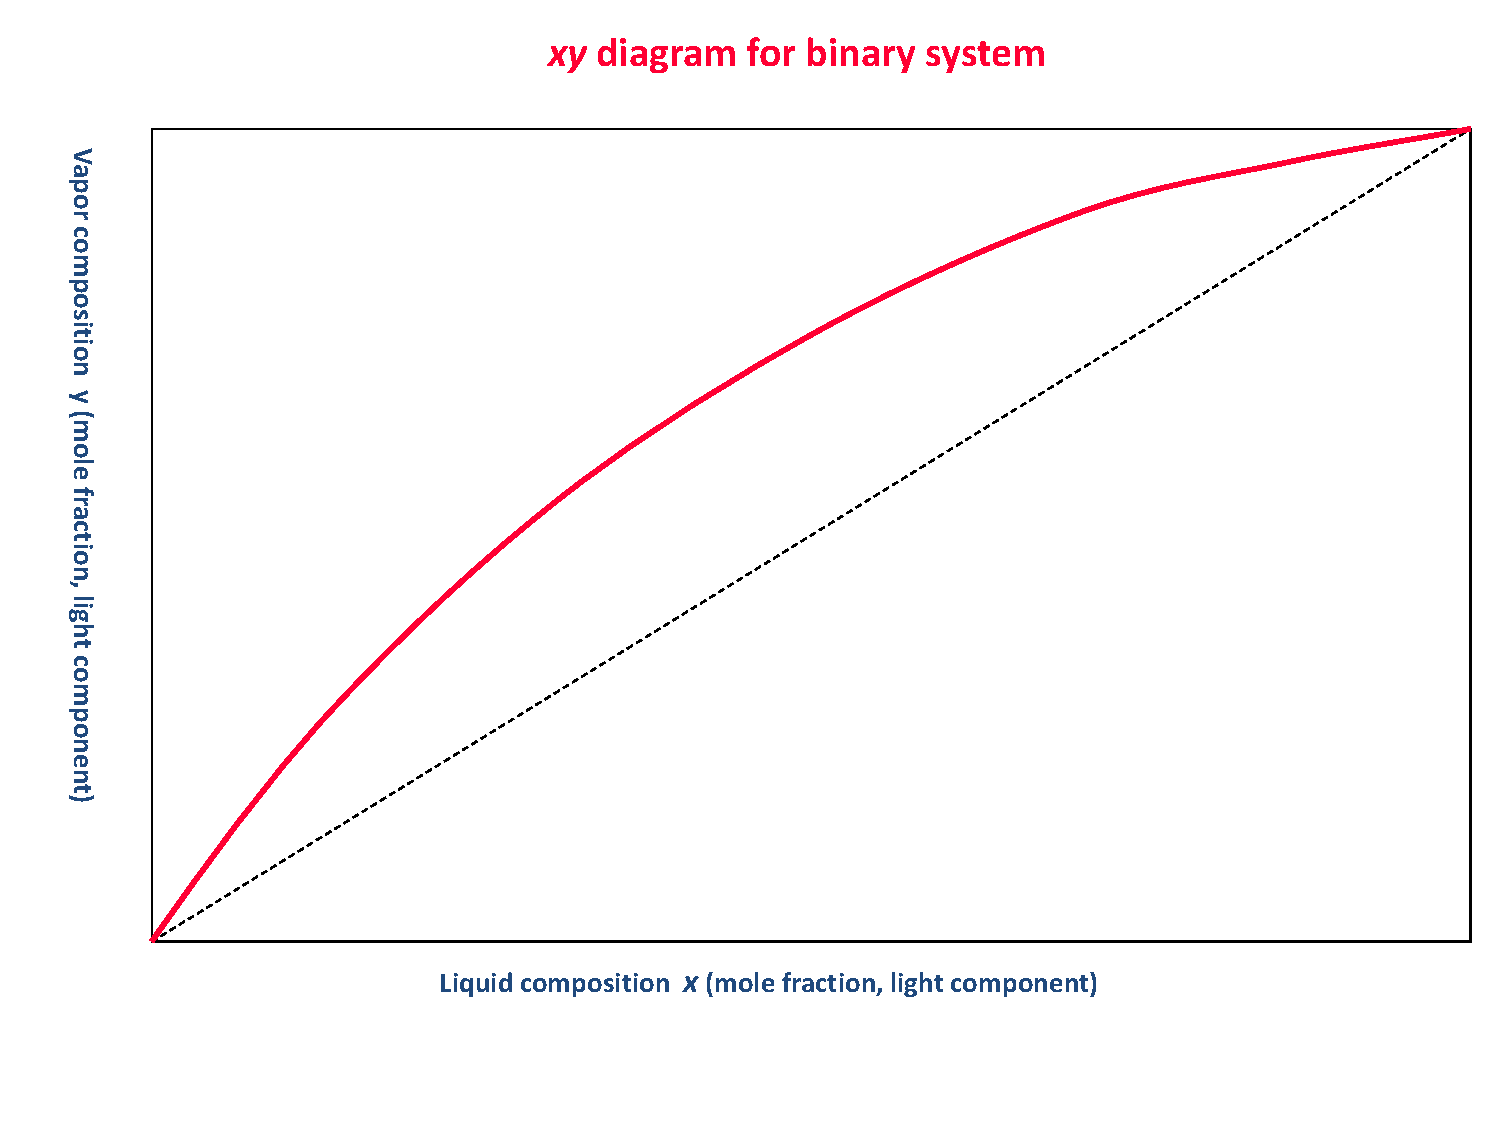
\includegraphics[width=5.5cm,height=4.cm,clip]{./../Pics/VLE_xy_DiagramIdeal}} \hspace{1cm}
           \visible<2->{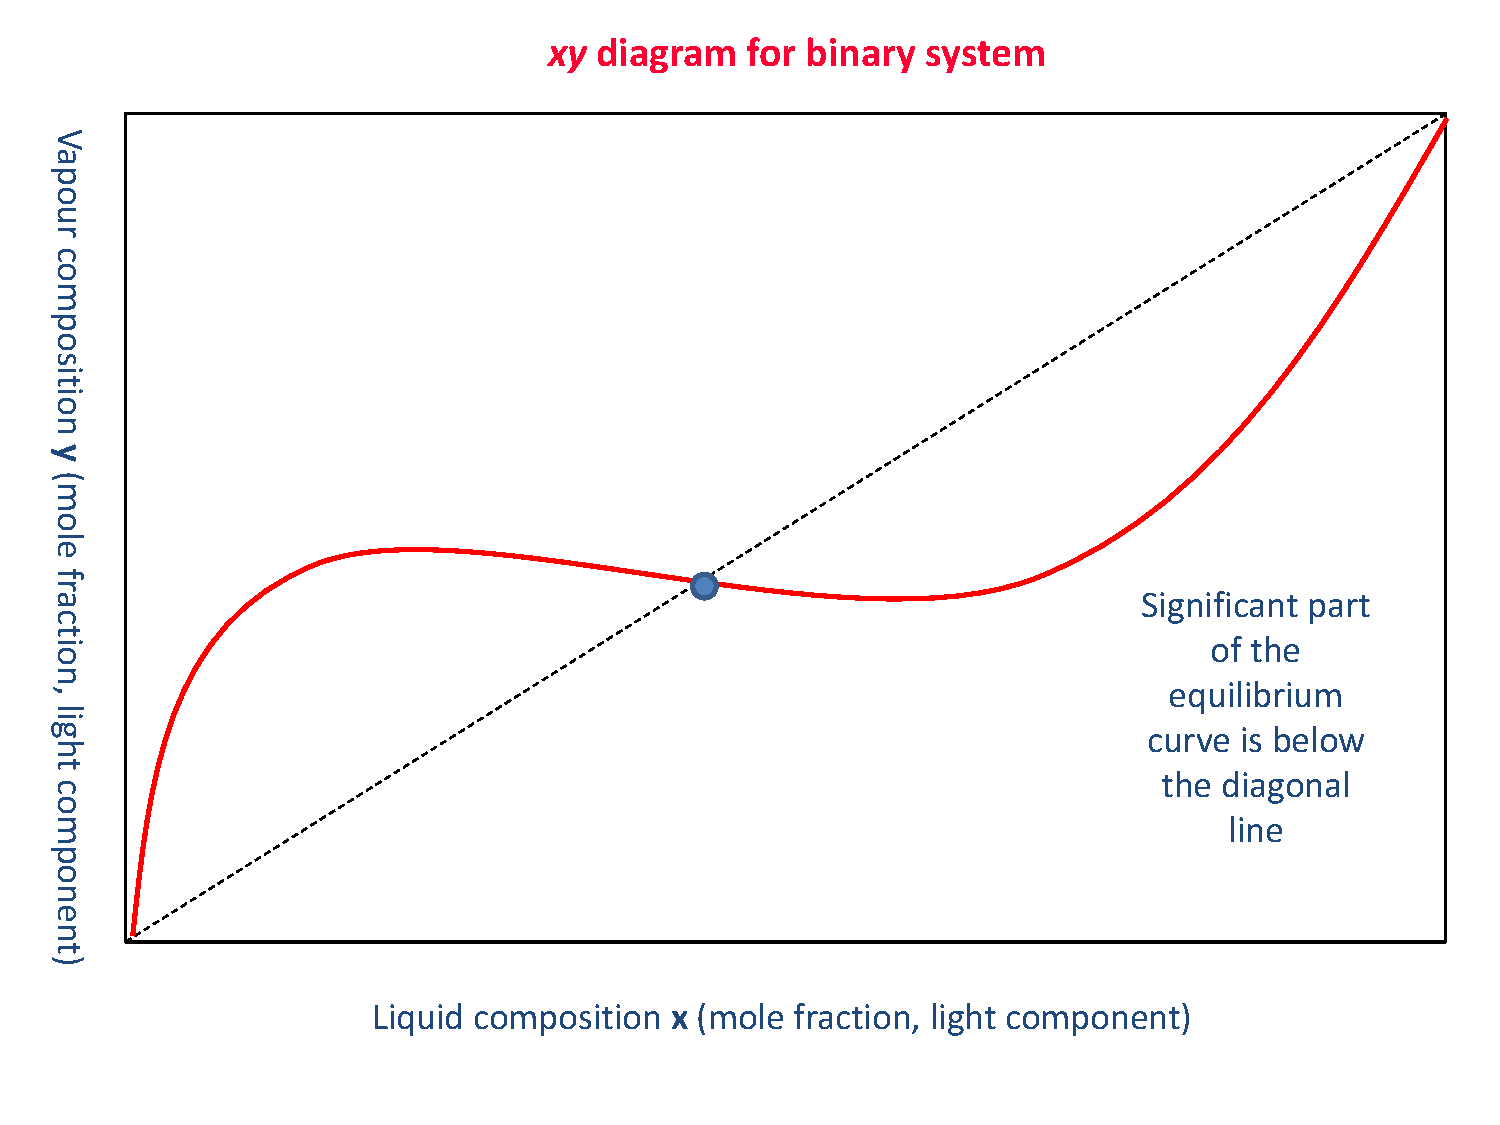
\includegraphics[width=5.5cm,height=4.cm,clip]{./../Pics/VLE_xy_DiagramNonIdeal1}}}
  \vspace{-0.2cm}
  \hbox{\hspace{4cm}
        \visible<3->{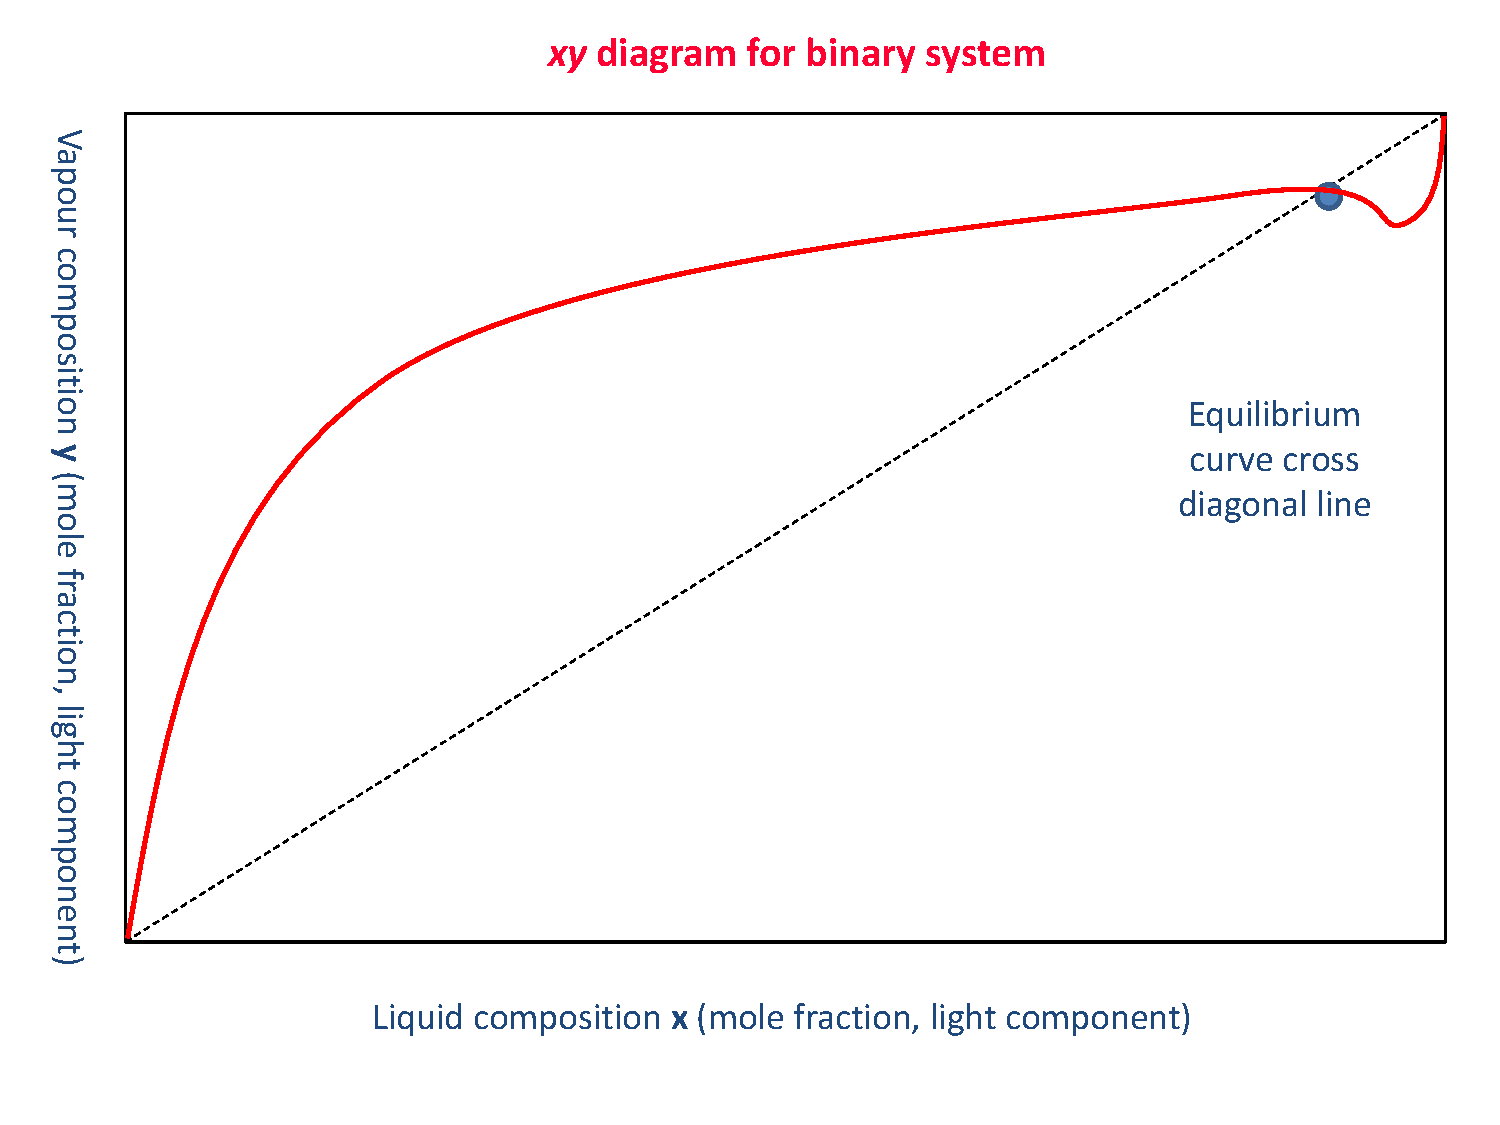
\includegraphics[width=5.5cm,height=4.cm,clip]{./../Pics/VLE_xy_DiagramNonIdeal2}}}
  }
\end{frame}
\normalsize


%%%
%%% SUBSECTION
%%%
\subsection{Activity}
%%%
%%% Slide
%%%
%\scriptsize
\begin{frame}
  \frametitle{Activity: An Assessment Tool of Ideality of Mixtures}
        \begin{enumerate}%\setcounter{enumi}{3}  
           \item<1-> Let's consider a liquid mixture with
               \begin{displaymath}
                  \mu_{i} = RT\ln{\overline{f}_{i}} + C_{i}(T), \text{ with } i=1, 2, \cdots, \mathcal{C}.
               \end{displaymath}
           \item<2-> Also, let's consider the same fluid $i$ pure at a \blue{reference-state}, \ie at $T$ and reference-state pressure, $P_{\text{ref}}$. If we subtract the chemical potential of $i$ at the reference-state $\left(\mu_{i}^{\circ}\right)$ from the mixture,
               \begin{displaymath}
                  \mu_{i} - \mu_{i}^{\circ} = RT\ln{\left(\frc{\overline{f}_{i}}{f_{i}^{\circ}}\right)} , \text{ with } i=1, 2, \cdots, \mathcal{C},
               \end{displaymath}
               where $f_{i}^{\circ}$ is the fugacity of component $i$ pure at \blue{reference-state} conditions.
           
           \visible<3->{\begin{block}{\begin{center}\normalsize{Activity }\end{center}}
               The term in brackets is defined as the \red{activity $\left(a_{i}\right)$} of component $i$,
                    \begin{displaymath} 
                          a_{i} = \frc{\overline{f}_{i}}{f_{i}^{\circ}},
                    \end{displaymath}
                    which measures {\it deviation} from ideal behaviour of liquid solutions. 
               \end{block}}
               
        \end{enumerate}
\end{frame}
\normalsize


%%%
%%% SUBSECTION
%%%
\subsection{Activity Coefficient}

%%%
%%% Slide
%%%
%\scriptsize
\begin{frame}
  \frametitle{Activity Coefficient}
        \begin{enumerate}%\setcounter{enumi}{2}  
           \item<1-> Since the chemical potential was defined as the molar Gibbs free energy, at the \blue{reference-state} $\mu_{i}^{\circ} = \overline{g}_{i}^{\circ}$, therefore
              \begin{displaymath}
                 \mu_{i} = \overline{g}_{i}^{\circ} + RT\ln{a_{i}},
              \end{displaymath}
              where $\overline{g}_{i}^{\circ}$ is the molat Gibbs free energy of pure component $i$ at \blue{reference-state}. This is often tabulated for a number of chemical species and can be found in any ChemEng handbooks;
           
           \visible<2->{\begin{block}{\begin{center}\normalsize{ Activity Coefficient}\end{center}}
               For an \blue{ideal solution}, we can apply the \blue{Lewis-Randall rule}, 
                  \begin{displaymath}
                     a_{i} = \frc{\overline{f}_{i}}{f_{i}^{\circ}} = \frc{y_{i}f_{i}}{f_{i}^{\circ}} \;\; \Longrightarrow \;\; \frc{f_{i}}{f_{i}^{\circ}} = \frc{a_{i}}{y_{i}} = \gamma_{i}
                  \end{displaymath}
                  and define the \red{activity coefficient $\left(\gamma_{i}\right)$}. The \blue{activity coefficient} is an {\it adjustment} parameter that \blue{relates the actual behaviour to the ideal behaviour of a solution at the same $T$ and $P$}. In a broad way, $\gamma$ operarates in a similar way as the compressibility factor ($Z$) for gases (Module 1).
                    
               \end{block}}
               
        \end{enumerate}
\end{frame}
\normalsize

%%%
%%% Slide
%%% 
%\scriptsize
\begin{frame}
  \frametitle{Activity Coefficient}
       \begin{block}{\begin{center}\normalsize{ Activity Coefficient}\end{center}}
            \begin{enumerate}\setcounter{enumi}{1}  
               \item<1-> For solutions
                  \begin{displaymath}
                     \gamma_{i} = \frc{\overline{f}_{i}}{x_{i}f_{i}}
                  \end{displaymath}
               \item<2-> For VLE at low pressures:
                  \begin{eqnarray}
                      \red{\gamma_{i}} &=& \frc{\overline{f}_{i}}{x_{i}f_{i}} = \frc{y_{i}P}{x_{i}f_{i}} \nonumber \\
                                        &=&  \red{\frc{y_{i}P}{x_{i}P_{i}^{\text{sat}}}}, \nonumber
                  \end{eqnarray}
                  this expression is the \red{modified Raoult's law}, defined in Module 3.
             \end{enumerate}
        \end{block}
         
\end{frame}
\normalsize


%%%
%%% SECTION
%%% 
\section{Solutions Theory}

%%%
%%% SUBSECTION
%%%
\subsection{Gibbs-Duhem Relations}

%\scriptsize
\begin{frame}
  \frametitle{Gibbs-Duhem Relations}
  \begin{enumerate}%\setcounter{enumi}{8}
    \item<1->For the total property $M\;(\equiv V,U,H,S,A,G)$:
      \visible<1->{\begin{displaymath}
          n M = \sum\limits_{i} n_{i}\overline{M}_{i} \Longrightarrow M = \sum\limits_{i}x_{i}\overline{M}_{i}, \text{ where }\;\overline{M}_{i}=\Partial[\left(nM\right)]{n_{i}}{P,T,n_{j} \left(n_{i} \ne n_{j}\right)  }
      \end{displaymath}
      is the partial molar property of species $i$ in solution.}
    \item<2->General expression for $dM$:
      \visible<2->{\begin{displaymath}
          dM = \sum\limits_{i}x_{i}d\overline{M}_{i} + \sum\limits_{i}\overline{M}_{i}dx_{i}
      \end{displaymath}}
  \end{enumerate}
  \visible<3->{\begin{block}{\begin{center}\normalsize{Gibbs-Duhem Equation }\end{center}}
               \begin{displaymath}
                   \red{\left(\frc{\partial M}{\partial P}\right)_{T,x} dP + \left(\frc{\partial M}{\partial T}\right)_{P,x}dT - \sum\limits_{i}x_{i}d\overline{M}_{i} = 0}
                \end{displaymath}
               and at $T$ and $P$ constant:
               \begin{displaymath}
                  \red{\sum\limits_{i}x_{i}d\overline{M}_{i} = 0}
               \end{displaymath}
             \end{block}}
\end{frame}
\normalsize

%%%
%%% Slide
%%%
%\scriptsize
\begin{frame}
  \frametitle{Partial Properties in Binary Solutions}
    \begin{block}{\begin{center}\normalsize{Applications of the Gibbs-Duhem Equation }\end{center}}
      \begin{enumerate}%\setcounter{enumi}{8}
         \item<1->Partial properties are readily calculated directly from an expression of the solution property as a function of composition at constant $T$ and $P$:
            \visible<1->{\begin{displaymath}
                            \red{\overline{M}_{1} = M + x_{2}\frc{d M}{dx_{1}} \;\;\;\text{ and } \;\;\; \overline{M}_{2}=M-x_{1}\frc{d M}{dx_{1}}}
                         \end{displaymath}}
         \item<2->Or in derivative format:
            \visible<2->{\begin{displaymath}
                            \blue{x_{1}\frc{d\overline{M}_{1}}{dx_{1}} + x_{2}\frc{d\overline{M}_{2}}{dx_{1}} = 0\;\;\;\text{ and }\;\;\; \frc{d\overline{M}_{1}}{dx_{1}} = -\frc{x_{2}}{x_{1}}\frc{d\overline{M}_{2}}{dx_{1}}}
                         \end{displaymath}}
      \end{enumerate}
   \end{block}
\end{frame}
\normalsize



%%%
%%% SUBSECTION
%%5
\subsection{Ideal Gas Mixture Model}

%%%
%%% Slide
%%%
%\scriptsize
\begin{frame}
  \frametitle{Ideal Gas Mixture Model}
  \begin{enumerate}
    \item<1->Useful model:
        \begin{enumerate}
          \item<1->Has a molecular basis;
          \item<1-> Approximates reality in well-defined limit of zero pressure;
          \item<1-> is analytically simple.
        \end{enumerate}
    \item<2-> Partial pressure:
        \visible<2->{\begin{displaymath}
            P_{i} = \frc{y_{i}R T}{V^{\text{ig}}} = y_{i}P\;\;\;\;\;\left(i=1,2,\cdots,\mathcal{N}\right)
        \end{displaymath} }
  \end{enumerate}
  \visible<3->{\begin{block}{\textcolor{blue}{Gibbs Theorem}}
                  \textcolor{blue}{$\lq$A partial molar property of a constituent species in an ideal-gas mixture is equal to the corresponding molar property of the species as a pure ideal gas at the mixture $T$ but at a $P$ equal to its partial pressure in the mixture.'\begin{displaymath}
            \overline{M}^{\text{ig}}_{i}\left(T,P\right) = M^{\text{ig}}_{i}\left(T,P_{i}\right)
          \end{displaymath}}
               \end{block}}
\end{frame}
\normalsize


%%%
%%% Slide
%%%
%\scriptsize
\begin{frame}
  \frametitle{Ideal Gas Mixture Model}
  \begin{enumerate}\setcounter{enumi}{2}
      \item<1->Properties of ideal-gas mixtures:
          \visible<1->{\begin{eqnarray}
             \blue{H^{\text{ig}} = \sum\limits_{i} y_{i}H_{i}^{\text{ig}}}, &&\blue{S^{\text{ig}} = \sum\limits_{i} y_{i}S_{i}^{\text{ig}}-R\sum\limits_{i}y_{i}\ln y_{i}}\;\;\; \nonumber \\
             && \blue{G^{\text{ig}}=\sum\limits_{i}y_{i}G_{i}^{\text{ig}} + RT\sum\limits_{i}y_{i}\ln y_{i}}\nonumber
          \end{eqnarray}}
      \item<2-> The Gibbs energy for ideal gas at constant $T$:
          \visible<2->{\begin{displaymath}
              \blue{ dG_{i}^{\text{ig}} = V_{i}^{\text{ig}} dP = \frc{RT}{P}dP = RT d\ln P}
          \end{displaymath}}
      \item<3-> And after integration:
          \visible<3->{\begin{displaymath}
              \blue{\mu^{\text{ig}} = \overline{G}_{i}^{\text{ig}}=\Gamma_{i}\left(T\right)+RT d\ln\left(y_{i}P\right)}\;\;\;\blue{G^{\text{ig}} =\sum\limits_{i}y_{i}\Gamma_{i}\left(T\right) + RT\sum\limits_{i}y_{i}\ln\left(y_{i}P\right)}
          \end{displaymath}}
  \end{enumerate}
\end{frame}
\normalsize


%%%
%%% FUGACITY
%%%
\subsection{Fugacity}

%%%
%%% Slide
%%%
%\scriptsize
\begin{frame}
  \frametitle{Fugacity and Fugacity Coefficient in Pure Species}
  \begin{enumerate}%\setcounter{enumi}{2}
      \item<1-> The \blue{chemical potential, $\mu$} and \blue{fugacity, $f$} for pure species and mixtures are related from,
          \visible<1->{\begin{displaymath}
             \frc{G_{i}}{n} = \mu_{i} = RT\ln f_{i} + \mathcal{C}_{i}, \;\;\;\; f^{\text{ig}}_{i} = P 
          \end{displaymath}} 
      \item<2-> The fugacity coefficient is defined as \blue{$\phi_{i}=\frc{f_{i}}{P}$};
      \item<3-> Now we can re-define the \blue{residual Gibbs energy}:
          \visible<3->{\begin{displaymath}
              \blue{ G_{i}^{\text{R}} = G_{i}-G_{i}^{\text{ig}} = RT\ln\frc{f_{i}}{P} = RT\ln\phi_{i}}
          \end{displaymath}}
  \end{enumerate}
\end{frame}
\normalsize




%%%
%%% Slide
%%%
%\scriptsize
\begin{frame}
  \frametitle{Fugacity and Fugacity Coefficient in VLE of Pure Species}
  \begin{enumerate}%\setcounter{enumi}{2}
      \item<1-> Saturated vapour and saturated liquid in equilibrium:
          \visible<1->{\begin{displaymath}
             G_{i}^{k} = \mathcal{C}_{i}\left(T\right)+ RT\ln f_{i}^{k}\;\;\;\left(\text{ with } k=\text{liquid, vapour}\right)\;\;\text{ and } f_{i}^{\text{v}}=f_{i}^{\text{l}}=f_{i}^{\text{sat}}
          \end{displaymath}} 
          \visible<2->{\blue{The vapour and liquid phases of pure chemical species are in equilibrium when both phases have the same temperature, pressure and} \red{fugacity}.} 
      \item<3-> Fugacity of pure liquid:
          \visible<3->{\begin{displaymath}
             f_{i}^{\text{l}}\left(P\right) = \frc{f_{i}^{\text{v}}\left(P_{i}^{\text{sat}}\right)}{P_{i}^{\text{sat}}} \frc{f_{i}^{\text{l}}\left(P_{i}^{\text{sat}}\right)}{f_{i}^{\text{v}} \left(P_{i}^{\text{sat}}\right)} \frc{f_{i}^{\text{l}}\left(P\right)}{f_{i}^{\text{l}}\left(P_{i}^{\text{sat}}\right)}P_{i}^{\text{sat}}\;\; \red{\Longrightarrow}\;\; \blue{f_{i}^{\text{l}} = \phi_{i}^{\text{sat}}P_{i}^{\text{sat}} \exp\left[\frc{V_{i}^{\text{l}}\left(P-P_{i}^{\text{sat}}\right)}{RT}\right]}
          \end{displaymath}
          where $V_{i}^{\text{l}}$ is assumed constant. The exponential term is also known as \blue{Poynting factor}.
}
  \end{enumerate}
\end{frame}
\normalsize

%%%
%%% Slide
%%%
%\scriptsize
\begin{frame}
  \frametitle{Fugacity and Fugacity Coefficient of Species in Solution}
  \begin{enumerate}%\setcounter{enumi}{2}
      \item<1-> For species $i$ in a mixture of \blue{real gases} or \blue{liquids (solution)}:
          \visible<1->{\begin{displaymath}
             \mu_{i} = \mathcal{C}_{i}\left(T\right) + RT\ln\overline{f}_{i}
          \end{displaymath}
          where $\overline{f}_{i}$ represents the fugacity of component $i$ in the mixture.} 
      \item<2-> Therefore, for an arbitrary number of phases $\left(\mathcal{P}=\alpha,\beta,\cdots,\pi\right)$ in equilibrium:
          \visible<2->{\begin{displaymath}
             \overline{f}_{i}^{\alpha} = \overline{f}_{i}^{\beta} = \cdots = \overline{f}_{i}^{\pi} \;\;\;\text{ with } i = 1,2,3,\cdots,\mathcal{N} 
          \end{displaymath}}
          \visible<3->{\blue{Multiple phases at the same $T$ and $P$ are in equilibrium when the fugacity of each component (i.e., chemical species) is the same in {\bf all phases}. }}
      \item<4-> \blue{Fugacity coefficient} for species in solution: \blue{$\overline{\phi}_{i}=\frc{\overline{f}_{i}}{y_{i}P}$}.
  \end{enumerate}
\end{frame}
\normalsize

%%%
%%% SUBSECTION
%%%
\subsection{Ideal Solution Model}

%%%
%%% Slide
%%%
%\scriptsize
\begin{frame}
  \frametitle{Ideal Solution Model}
  \begin{enumerate}%\setcounter{enumi}{2}
      \item<1->\blue{A solution is ideal (id) when:} 
          \visible<1->{\begin{displaymath}
             \blue{\mu_{i}^{\text{id}} = \overline{G}_{i}^{\text{id}} = G_{i}\left(T,P\right) + RT\ln x_{i}}
          \end{displaymath}}
      \item<2-> Total values of properties:
          \visible<2->{\begin{eqnarray}
             G^{\text{id}} = \sum\limits_{i}x_{i}G_{i} + RT\sum\limits_{i}x_{i}\ln x_{i}, && S^{\text{id}} = \sum\limits_{i}x_{i}S_{i}-R\sum\limits_{i}x_{i}\ln x_{i} \nonumber \\
              V^{\text{id}} = \sum\limits_{i}x_{i}V_{i}   && H^{\text{id}} = \sum\limits_{i}x_{i}H_{i} \nonumber
          \end{eqnarray}}
      \item<3-> \blue{Lewis-Randall rule}:
          \visible<3->{\begin{displaymath}
             \mu_{i}=\mathcal{C}_{i}\left(T\right)+RT\ln\overline{f}_{i} \;\;\text{ and } \;\; G_{i}=\mathcal{C}_{i}\left(T\right)+RT\ln f_{i}
          \end{displaymath}
          led to 
          \begin{displaymath}
             \blue{\overline{f}_{i}^{\text{id}}=x_{i}f_{i}}
          \end{displaymath}}
  \end{enumerate}
\end{frame}
\normalsize


%%%
%%% SUBSECTION
%%%
\subsection{Excess Properties}

%%%
%%% Slide
%%%
%\scriptsize
\begin{frame}
  \frametitle{Excess Properties}
  \begin{enumerate}%\setcounter{enumi}{2}
      \item<1-> If $M$ represents the molar (or unit-mass) value of any extensive thermodynamic property (e.g., $V$, $U$, $H$, $G$,$S$ etc) then an \blue{excess property, $M^{\text{E}}$} is defined as
          \visible<1->{\begin{displaymath}
             M^{\text{E}} = M - M^{\text{id}}
          \end{displaymath}
          where $M$ and $M^{\text{id}}$ are the actual and ideal solution property.}
      \item<2-> \blue{This means the change in $M$ that occurs on mixing at constant $T$ and $P$ in addition to that which would occur if an ideal mixture were formed.}
      \item<3-> Excess properties are often complex non-linear functions of the composition, $T$ and $P$, and are usually obtained from experiments.
      \item<4-> Excess properties have \blue{no meaning} for pure species, whereas {\it residual properties} exist for both \red{pure species} and \red{mixtures}.
  \end{enumerate}
\end{frame}
\normalsize


%%%
%%% Slide
%%%
%\scriptsize
\begin{frame}[label={ExcessProperty}]
  \frametitle{Excess Properties}
  \begin{enumerate}\setcounter{enumi}{4}
      \item<1->Fundamental excess property relation
          \visible<1->{\begin{displaymath}
             d\left(\frc{\red{n} G^{\text{E}}}{RT}\right) = \frc{nV^{\text{E}}}{RT}dP - \frc{nH^{\text{E}}}{RT^{2}}dT + \sum\limits_{i}\frc{\overline{G}_{i}^{\text{E}}}{RT}dn_{i}
          \end{displaymath}}
      \item<2->\label{activitycoefficient} Relation with \blue{activity coefficient, $\gamma_{i}$}:
           \visible<2->{\begin{displaymath}
              \gamma_{i} = \frc{\overline{f}_{i}}{x_{i}f_{i}} \hspace{1cm}\red{\Longrightarrow}\hspace{1cm} \overline{G}_{i}^{\text{E}}=RT\ln\gamma_{i}
           \end{displaymath}}
      \item<3-> Effects of $P$ and $T$:
           \visible<3->{\begin{displaymath}
              \left(\frc{\partial\ln\gamma_{i}}{\partial P}\right)_{T,x}=\frc{\overline{V}^{\text{E}}_{i}}{RT}, \hspace{1cm} \left(\frc{\partial\ln\gamma_{i}}{\partial T}\right)_{P,x}=-\frc{\overline{H}^{\text{E}}_{i}}{RT^{2}}
           \end{displaymath}}
      \item<4-> Gibbs-Duhem equations
           \visible<4->{\begin{displaymath}
              \frc{G^{\text{E}}}{RT} = \sum\limits_{i}x_{i}\ln\gamma_{i}, \hspace{1cm} \left[\sum\limits_{i}x_{i}d\left(\ln\gamma_{i}\right)\right]_{T,P}=0
           \end{displaymath}}
  \end{enumerate}
\end{frame}
\normalsize

%%%
%%% Slide
%%%
%\scriptsize
\begin{frame}
  \frametitle{Excess Properties}
  \begin{enumerate}\setcounter{enumi}{8}
      \item<1-> Excess properties can be determined via
         \begin{enumerate}
            \item<1-> $G^{\text{E}}$ from VLE data;
            \item<1-> $H^{\text{E}}$ from mixing experiments;
            \item<1-> $S^{\text{E}}$ from $S^{\text{E}}=\frc{H^{\text{E}}-G^{\text{E}}}{T}$
         \end{enumerate}
      \item<2-> All excess properties become zero as either species approaches purity $\left(\text{i.e.,} x_{i}\rightarrow 1\right)$.
      \item<3-> Excess properties approach zero for ideal solutions, but thermodynamic properties might still change upon mixing
         \visible<3->{\begin{eqnarray}
             \Delta G^{\text{id}} = RT \sum\limits_{i} x_{i}\ln x_{i} && \Delta S^{\text{id}} = -R \sum\limits_{i} x_{i}\ln x_{i} \nonumber \\
             \Delta V^{\text{id}} = 0 && \Delta H^{\text{id}} = 0 \nonumber
         \end{eqnarray}}
  \end{enumerate}
\end{frame}
\normalsize

%%%
%%% Slide 
%%%
\scriptsize
\begin{frame} 
  \frametitle{Excess Properties}
     \begin{center}
       \begin{figure}
         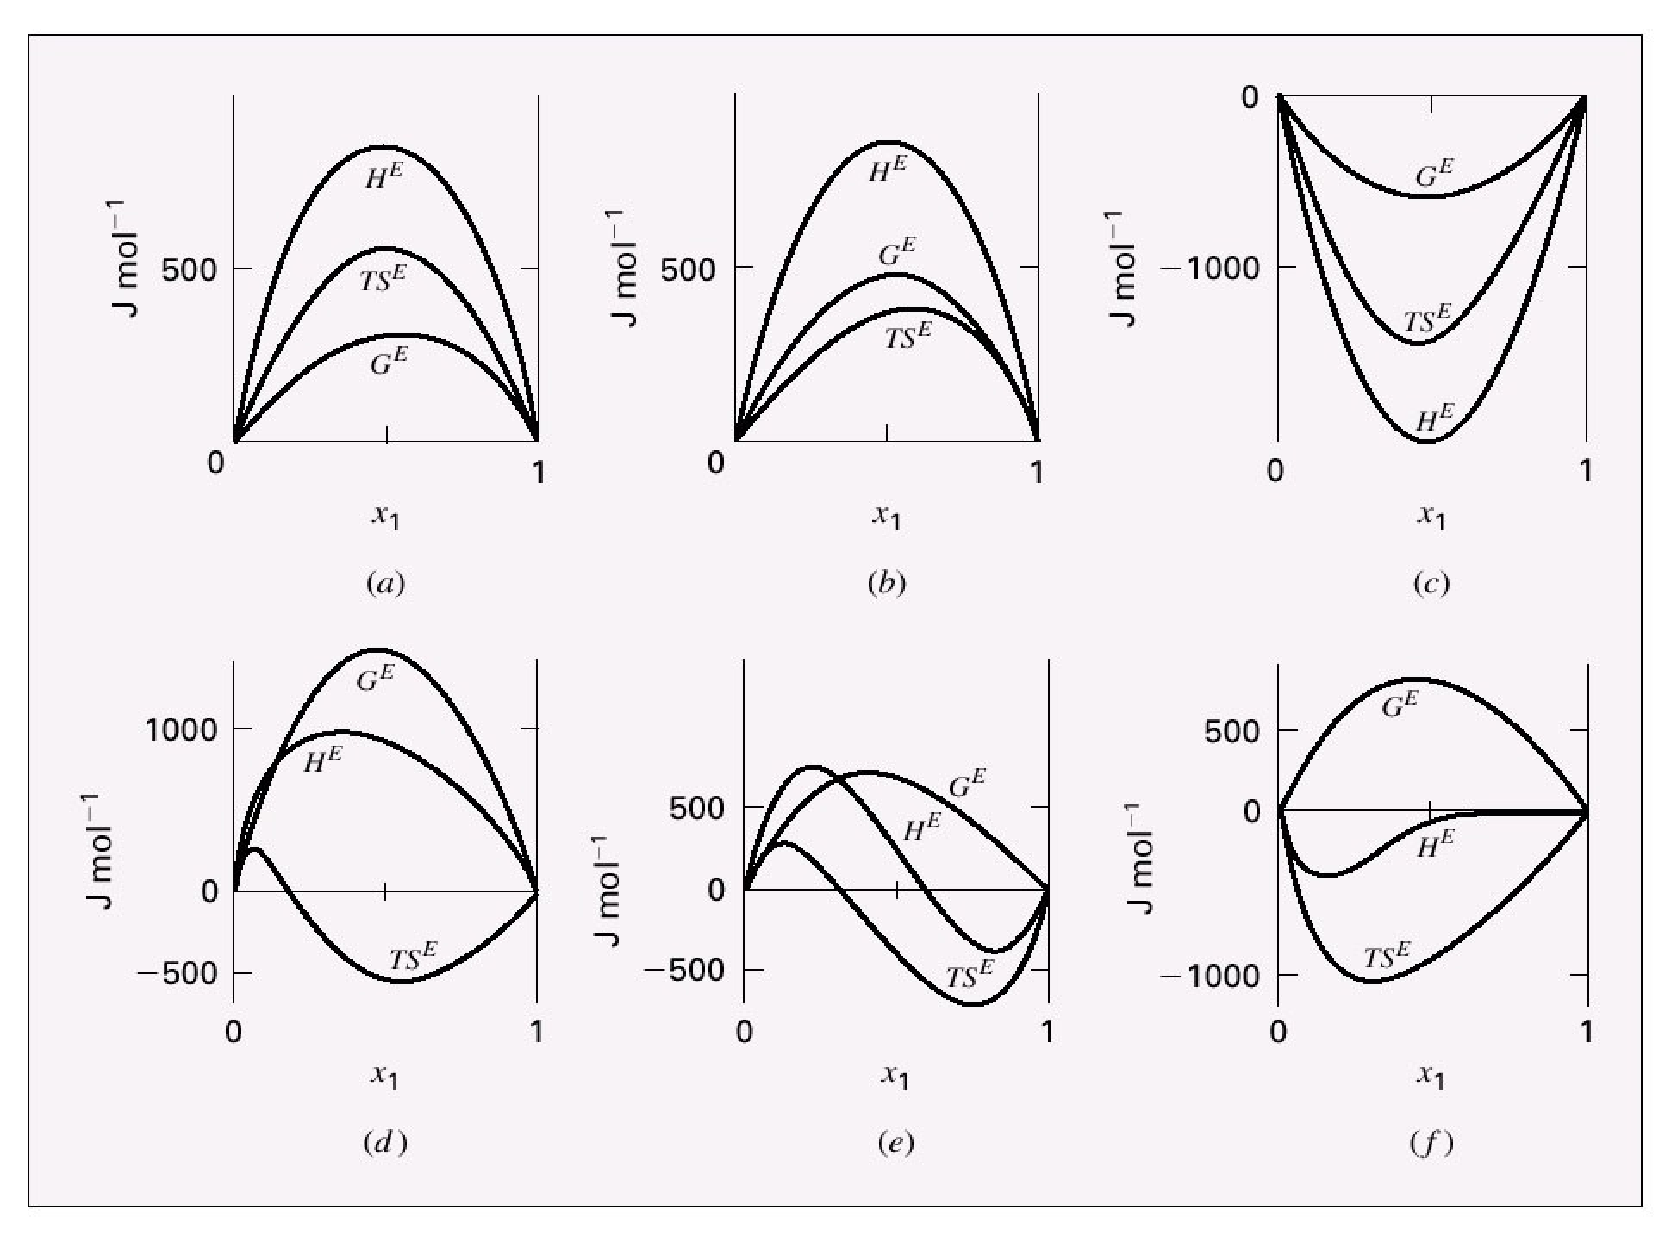
\includegraphics[width=9.cm, height=6.5cm,clip]{../Pics/ExcessProperties_Plot}
          \caption{\scriptsize Excess properties at 50$^{\circ}$C for the following binary liquid systems: (a) chloroform / n-heptane,(b) acetone / methanol, (c) acetone / chloroform, (d) ethanol / n-heptane, (e) ethanol / chloroform and (f) ethanol / water (Extracted from {\it Smith, Van Ness and Abott}). }
       \end{figure}
     \end{center}
\end{frame}
\normalsize


%%%
%%% SUBSECTION
%%%
\subsection{Activity Coefficient Models}

%%%
%%% Slide
%%%
%\scriptsize
\begin{frame}
  \frametitle{Activity Coefficient Models}
  \begin{enumerate}%\setcounter{enumi}{8}
      \item<1-> In several industrial and environmental applications EOS can not accurately predict the thermodynamic behaviour of solutions. In these cases, we can estimate the excess Gibbs energy \blue{$G^{\text{E}}$} (see Slide~\ref{ExcessProperty}, item~\ref{activitycoefficient}) by first calculating the activity coefficient, $\gamma_{i}$;
      \item<2-> Activity coefficient models are often more accurate (than traditional EOS) when strong intermolecular interactions are present;
      \item<3-> Models commonly used coefficient activity models in \blue{fluid simulators}:
          \begin{enumerate}
             \item<3-> Margules;
             \item<3-> Van Laar;
             \item<3-> Wilson;
             \item<3-> Non-Random-Two-Liquids (NRTL);
             \item<3-> UNIversal QUAsi Chemical (UNIQUAC).     
          \end{enumerate}
      \item<4-> Basic Equations:
          \visible<4->{\begin{displaymath}
            \gamma_{i} = \frc{\overline{f}_{i}}{x_{i}f_{i}}=\frc{\overline{f}_{i}}{\overline{f}_{i}^{\text{id}}},\hspace{1cm} \frc{G^{\text{E}}}{RT}=\xi\left(\gamma_{i}\right)
          \end{displaymath}
           where $\xi\left(\gamma_{i}\right)$ is a function of $\gamma_{i}$. Bear in mind that $\gamma_{i}$ is a function of composition, $x_{i}$. }
  \end{enumerate}
\end{frame}
\normalsize


%%%
%%% Slide
%%%
%\scriptsize
\begin{frame}
  \frametitle{Activity Coefficient Models}
  \begin{enumerate}\setcounter{enumi}{4}
      \item<1-> 2-parameter models for binary systems:
        \begin{enumerate}
          \item<1-> Mergules equations;
             \visible<1->{\begin{displaymath}
                \ln\gamma_{1}=x_{2}^{2}\left[A_{12}+2\left(A_{21}-A_{12}\right)x_{1}\right] \hspace{1cm} \ln\gamma_{2}=x_{1}^{2}\left[A_{21}+2\left(A_{12}-A_{21}\right)x_{2}\right]
             \end{displaymath}}
          \item<2-> Van Laar equations:
             \visible<2->{\begin{displaymath}
                \ln\gamma_{1}= B_{12}\left(1+\frc{B_{12}x_{1}}{A_{21}x_{2}}\right)^{-2}  \hspace{1cm} \ln\gamma_{2}= B_{21}\left(1+\frc{B_{21}x_{1}}{A_{12}x_{2}}\right)^{-2}
             \end{displaymath}}
          \item<3-> Wilson equations:
             \visible<3->{\begin{eqnarray}
                && \frc{G^{\text{E}}}{RT} = x_{1}\ln\left(x_{1}+x_{2}C_{12}\right) - x_{2}\ln\left(x_{2}+x_{1}C_{21}\right) \nonumber \\
                && \ln\gamma_{1}= -\ln\left(x_{1}+x_{2}C_{12}\right) + x_{2}\left(\frc{C_{12}}{x_{1}+x_{2}C_{12}}-\frc{C_{21}}{x_{2}+x_{1}C_{21}}\right)\nonumber \\
                && \ln\gamma_{2}= -\ln\left(x_{2}+x_{2}C_{21}\right) + x_{2}\left(\frc{C_{12}}{x_{1}+x_{2}C_{12}}-\frc{C_{21}}{x_{2}+x_{1}C_{21}}\right)\nonumber 
             \end{eqnarray}}
        \end{enumerate} 
  \end{enumerate}
\end{frame}
\normalsize


%%%
%%% Slide
%%%
%\scriptsize
\begin{frame}
  \frametitle{Activity Coefficient Models}
  \begin{enumerate}\setcounter{enumi}{5}
      \item<1-> NRTL and UNIQUAC are 3-parameter models that incorporate binary attraction/repulsion parameters of multiple chemical species;
       \item<2-> UNIFAC (UNIQUAC Functional-group Activity Coefficient) is a group contribution model that assign specific thermodynamic properties to functional group species, e.g., \red{$\cdot$CH$_{3}$}, \red{:CH$_{2}$}, \red{:COH}, \red{$\cdot$OH}, etc.
  \end{enumerate}
\end{frame}
\normalsize


%%%
%%% SUMMARY
%%%
\section{Summary}

%%%
%%% Slide
%%%
%\scriptsize
\begin{frame}
 \frametitle{Summary}
   \begin{enumerate}[(i)]
      \item Excess molar properties;
      \item Definition of activity,activity coefficient, fugacity, fugacity coefficient and chemical potential for pure species and mixtures;
      \item Brief description of activity coefficient models currently used in simulators.
   \end{enumerate}
\end{frame}


%%%
%%% EXAMPLES
%%%
\begin{comment}

%%%
%%%  SECTION
%%%
\section{Examples}

%%%
%%% Slide
%%%
%\scriptsize 
\begin{frame}
 \frametitle{Example 1}\label{Ex1}
    \blue{At 25$^{\circ}$C and atmospheric pressure, the volume change of mixing of a binary liquid mixture of species 1 and 2 is given by,}
       \begin{displaymath}
          \blue{\Delta V = x_{1}x_{2}\left(45x_{1}+25x_{2}\right)\;\;\;\;\text{ with }\;\;\;\left[\Delta V\right] = \text{cm}^{3}.\text{mol}^{-1}}
       \end{displaymath}
       \blue{with molar volumes of $V_{1} = 110\;\text{cm}^{3}.\text{mol}^{-1}$ and $V_{2} = 90\;\text{cm}^{3}.\text{mol}^{-1}$. Determine the partial molar volumes, $\overline{V}_{1}$ and $\overline{V}_{2}$, in a mixture containing 40$\%$-mol of species 1.}

\end{frame}

%%%
%%% Slide
%%%
%\scriptsize 
\begin{frame}
 \frametitle{Example 2}\label{Ex2}
    \blue{A process stream contains light species 1 and heavy species 2. A relatively pure liquid stream containing mostly 2 is obtained through a single-stage liquid/vapour separator. Specifications on the equilibrium composition are: $x_{1}$ = 0.002 and $y_{1}$ = 0.950. Assuming that the modified Raoult's law applies, }
\begin{displaymath}
  \blue{y_{i} P = x_{i}\gamma_{i}P_{i}^{\text{sat}}}
\end{displaymath} 
\blue{Determine $T$ and $P$ for the separator. Given the activity coefficients for the liquid phase,}
\begin{displaymath}
   \blue{\ln\gamma_{1} = 0.93x_{2}^{2} \;\;\;\;\;\text{ and }\;\;\;\;\;\ln\gamma_{2}=0.93x_{1}^{2}}
\end{displaymath}
\begin{displaymath}
    \blue{\ln P_{i}^{\text{sat}} = A_{i} - \frc{B_{i}}{T}\;\;\;\text{with [P] = bar and [T] = K}}
\end{displaymath} 
\blue{$A_{1}$ =10.08, $B_{1}$ = 2572.0 K, $A_{2}$ = 11.63 and $B_{2}$ = 6254.0 K.}

\end{frame}

%%%
%%% Slide
%%%
%\scriptsize 
\begin{frame}
 \frametitle{Example 3}\label{Ex3}
    \blue{The experimental value of the partial molar volume $\left(\text{cm}^{3}\text{.mol}^{-1}\right)$ of a aqueous solution of K$_{2}$SO$_{4}$ is given by}
                \begin{displaymath}
                   \blue{\overline{V}_{A} = 32.280 + 18.216 m^{1/2},}
                \end{displaymath} 
 \blue{where $m$ is the molality (= number of moles per kg of water) of the K$_{2}$SO$_{4}$ . Use the Gibbs-Duhem equation to derive an equation for the partial molar volume of water in the solution. Plot $\overline{V}_{i}\;\;\times m$, with $0.0\leq m\leq 0.1$. The molar volume of pure water at 298.15 K is 18.079 cm$^{3}$.mol$^{-1}$ and the molar mass of pure water is 18 g.mol$^{-1}$.}

\end{frame}

\end{comment}  
\end{document}
 
